\subsubsection{Màn hình 3}
\textbf{Mô tả:} Tính lương cho nhân viên trong khoảng thời gian được chọn.

Màn hình ban đầu. Hiện tại đang hiển thị bảng rỗng cho người dùng chưa chọn ngày bắt đầu và ngày kết thúc cho khoảng thời gian tính lương.
\begin{figure}[H]
    \centering
    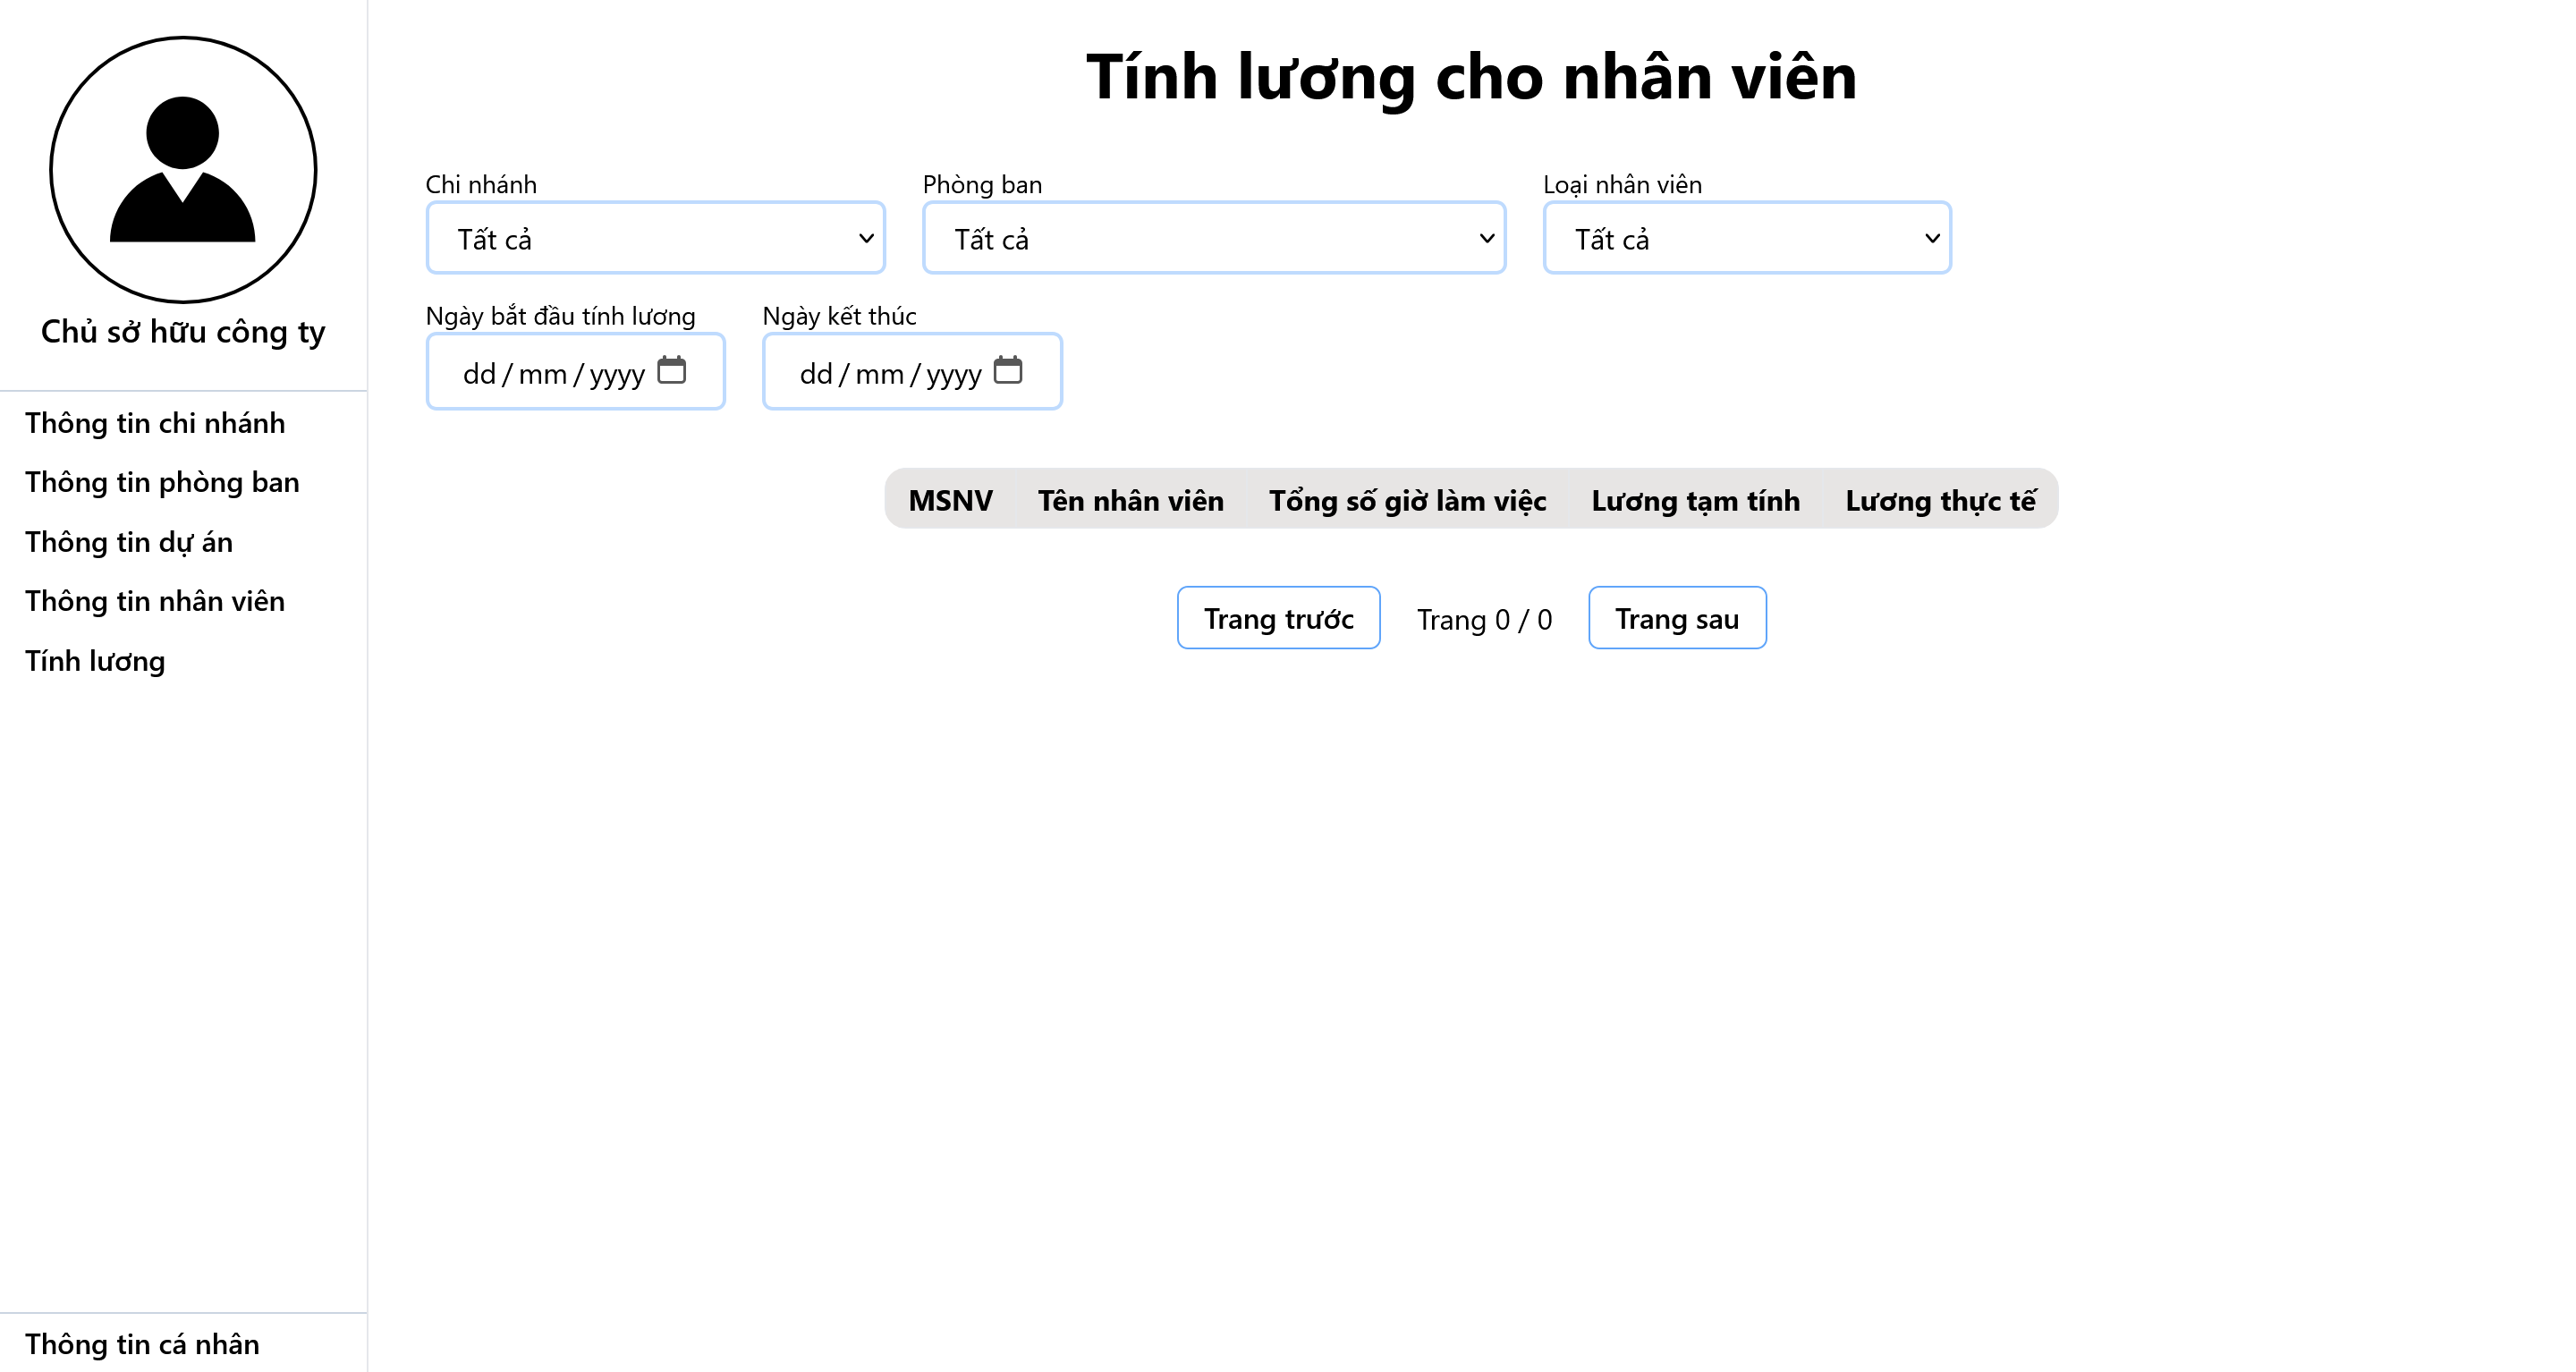
\includegraphics[width=1\linewidth]{content/images/ManHinh_3_a.png}
    \caption{Màn hình ban đầu, do chưa xác định thời gian nên hiện bảng rỗng}
    \label{fig:ManHinh_3_a}
\end{figure}

Sau khi người dùng chọn ngày bắt đầu và ngày kết thúc, màn hình sẽ hiển thị bảng lương của các nhân viên được lọc theo tiêu chí mà người dùng đặt.
\begin{figure}[H]
    \centering
    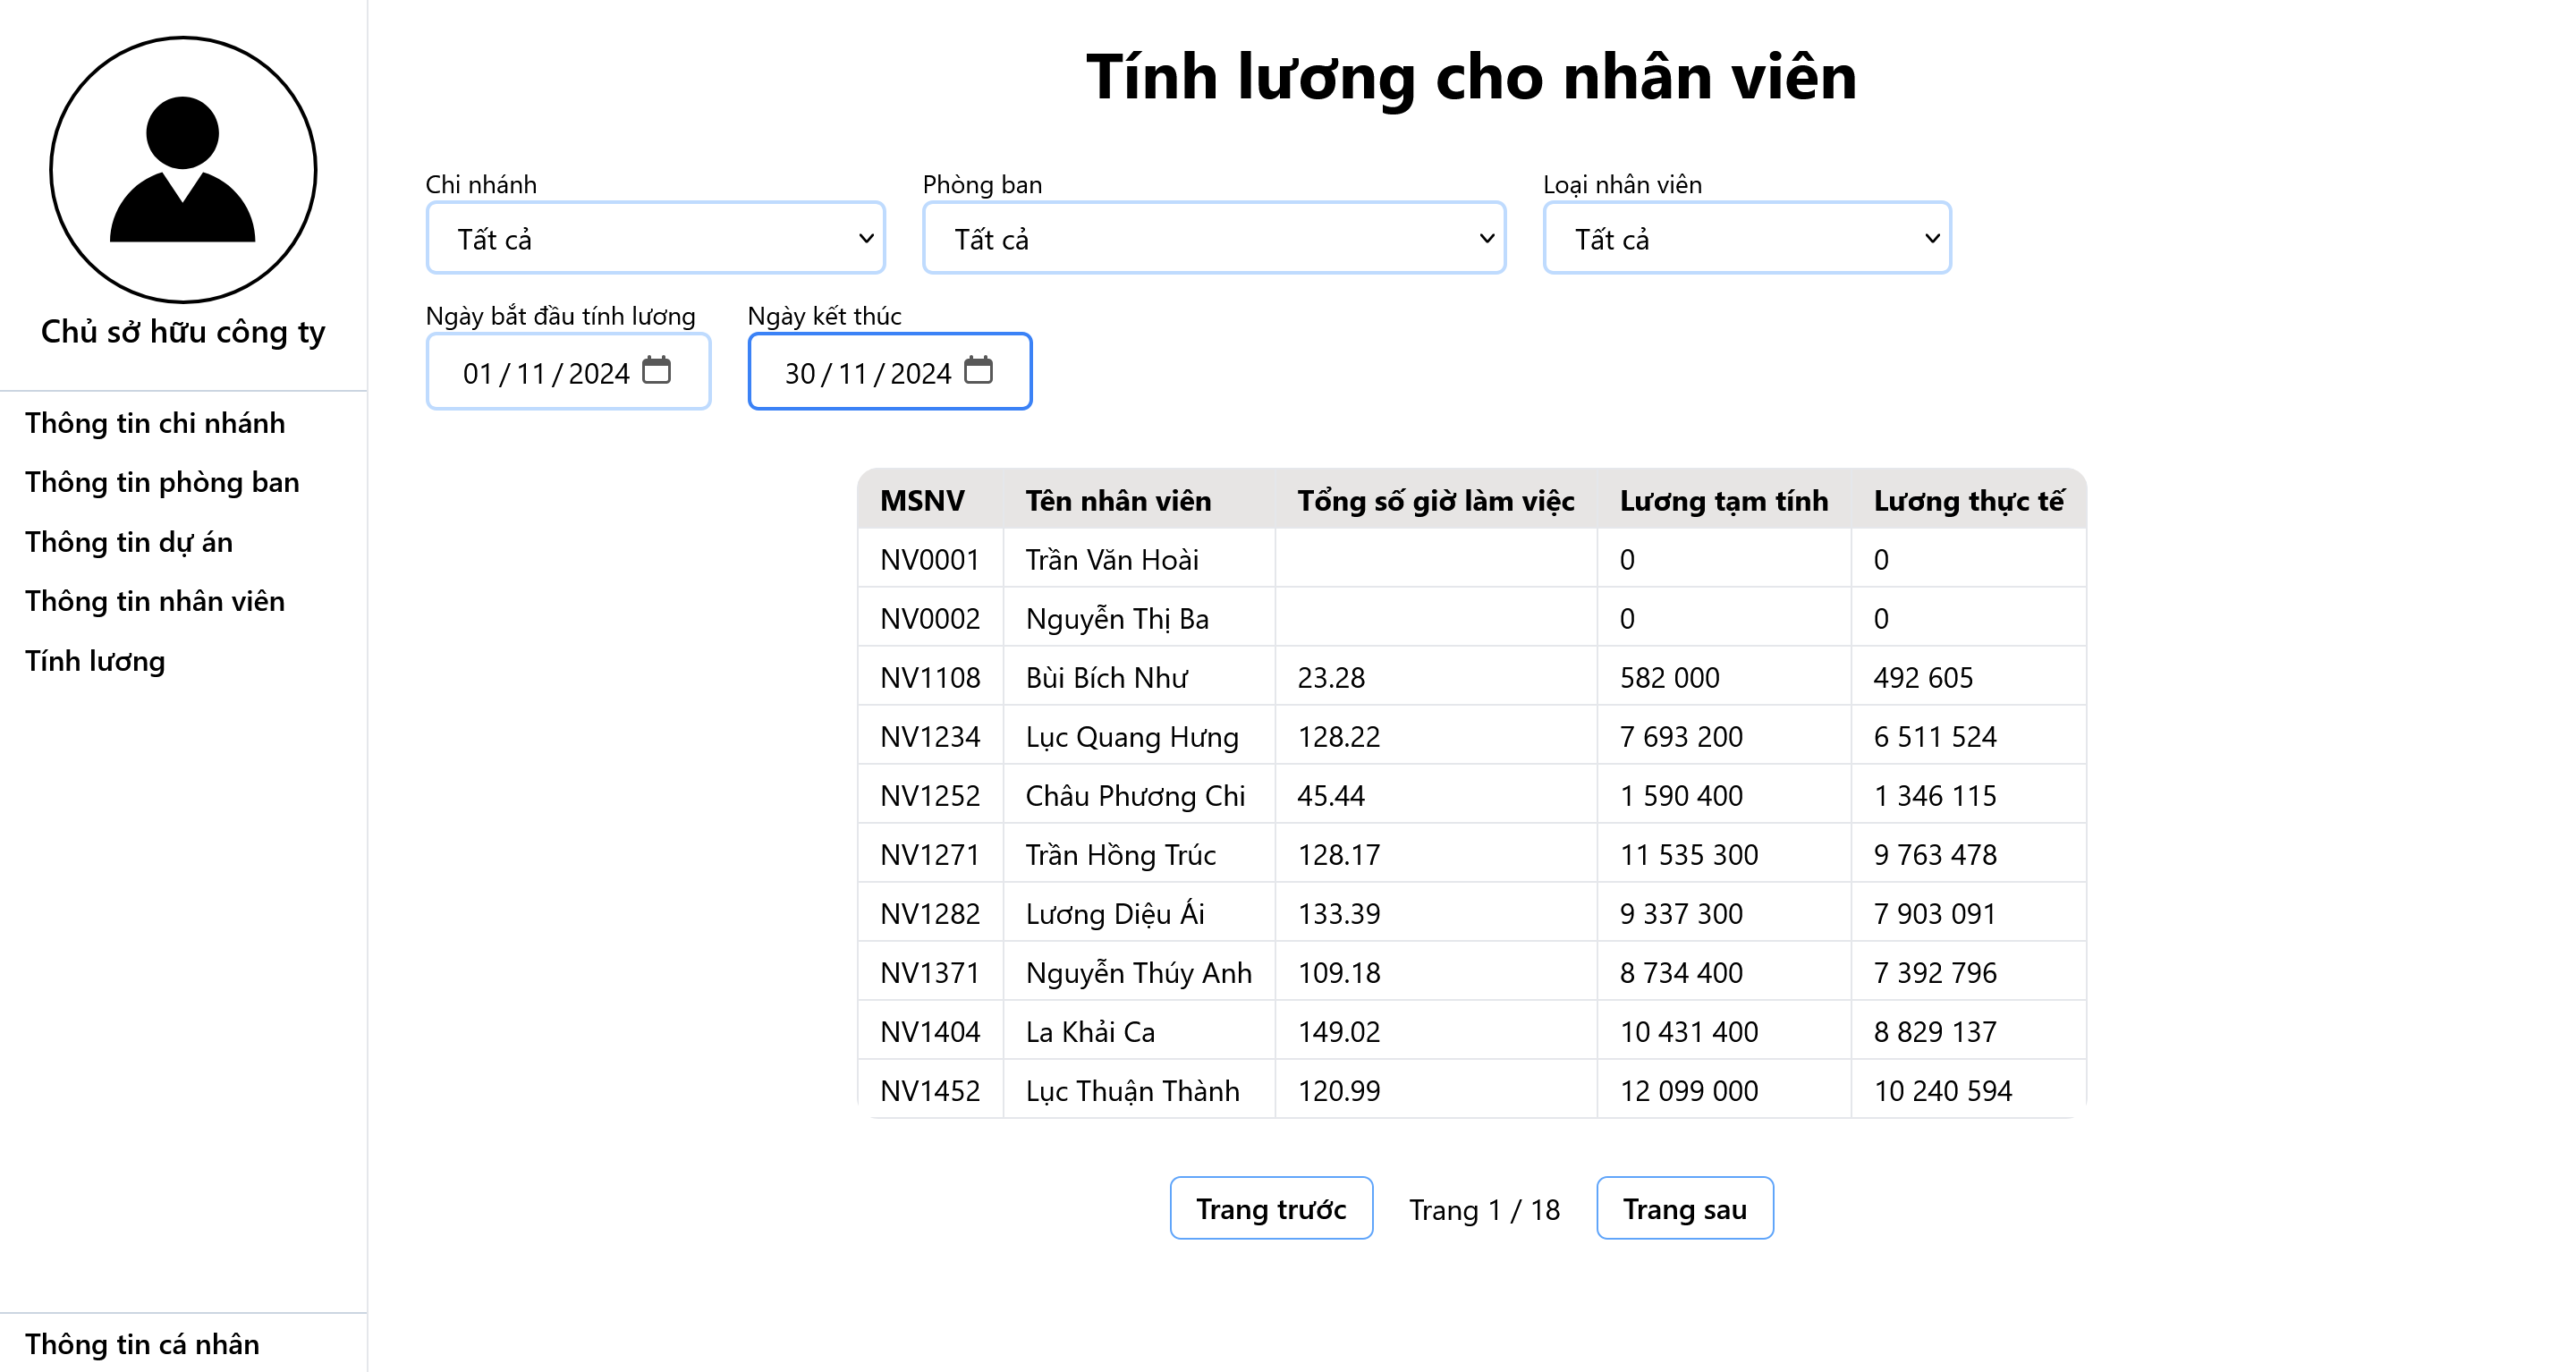
\includegraphics[width=1\linewidth]{content/images/ManHinh_3_b.png}
    \caption{Bảng lương của toàn bộ nhân viên tính từ ngày 01/11/2024 đến ngày 30/11/2024}
    \label{fig:ManHinh_3_b}
\end{figure}

Các tiêu chí mà người dùng có thể lọc nhân viên là:
\begin{itemize}
    \item [--] Lọc ra những nhân viên trong 1 phòng ban nào đóng
    \item [--] Lọc ra những nhân viên theo loại nhân viên (nhân viên toàn thời gian hoặc nhân viên bán thời gian)
\end{itemize}

Một vài màn hình ví dụ cho bộ lọc:
\begin{figure}[H]
    \centering
    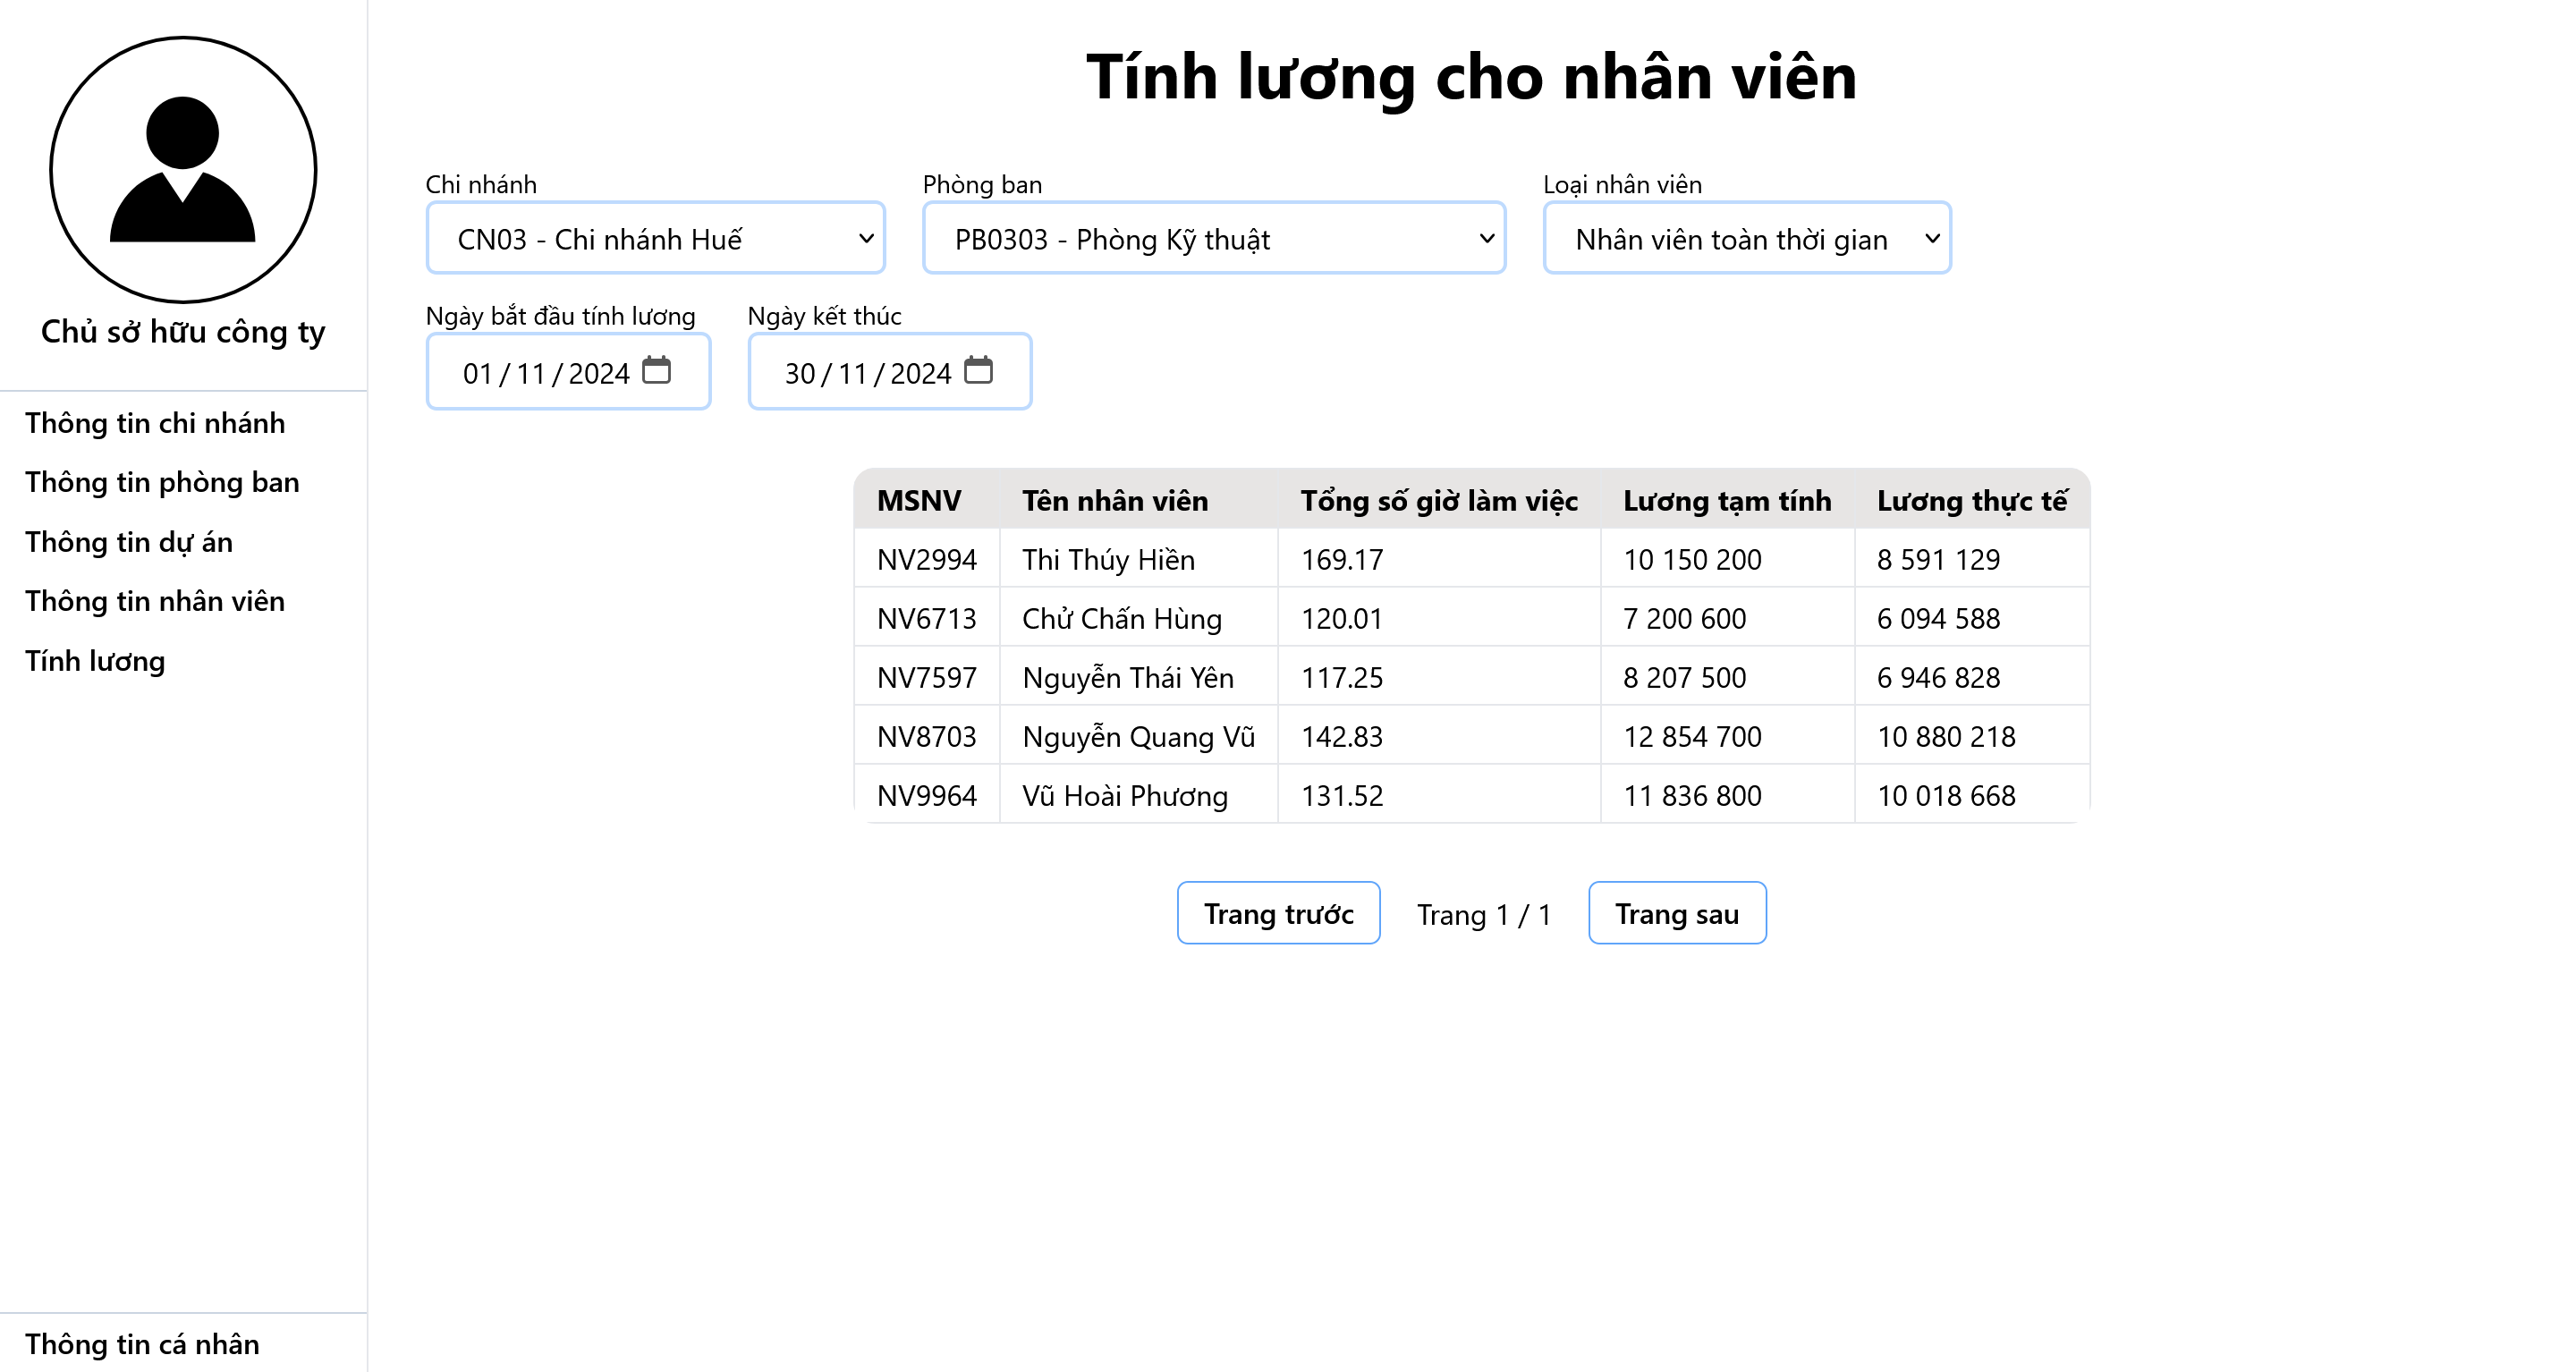
\includegraphics[width=1\linewidth]{content/images/ManHinh_3_c.png}
    \caption{Bảng lương của các nhân viên toàn thời gian thuộc phòng ban 'PB0303'}
    \label{fig:ManHinh_3_c}
\end{figure}

\begin{figure}[H]
    \centering
    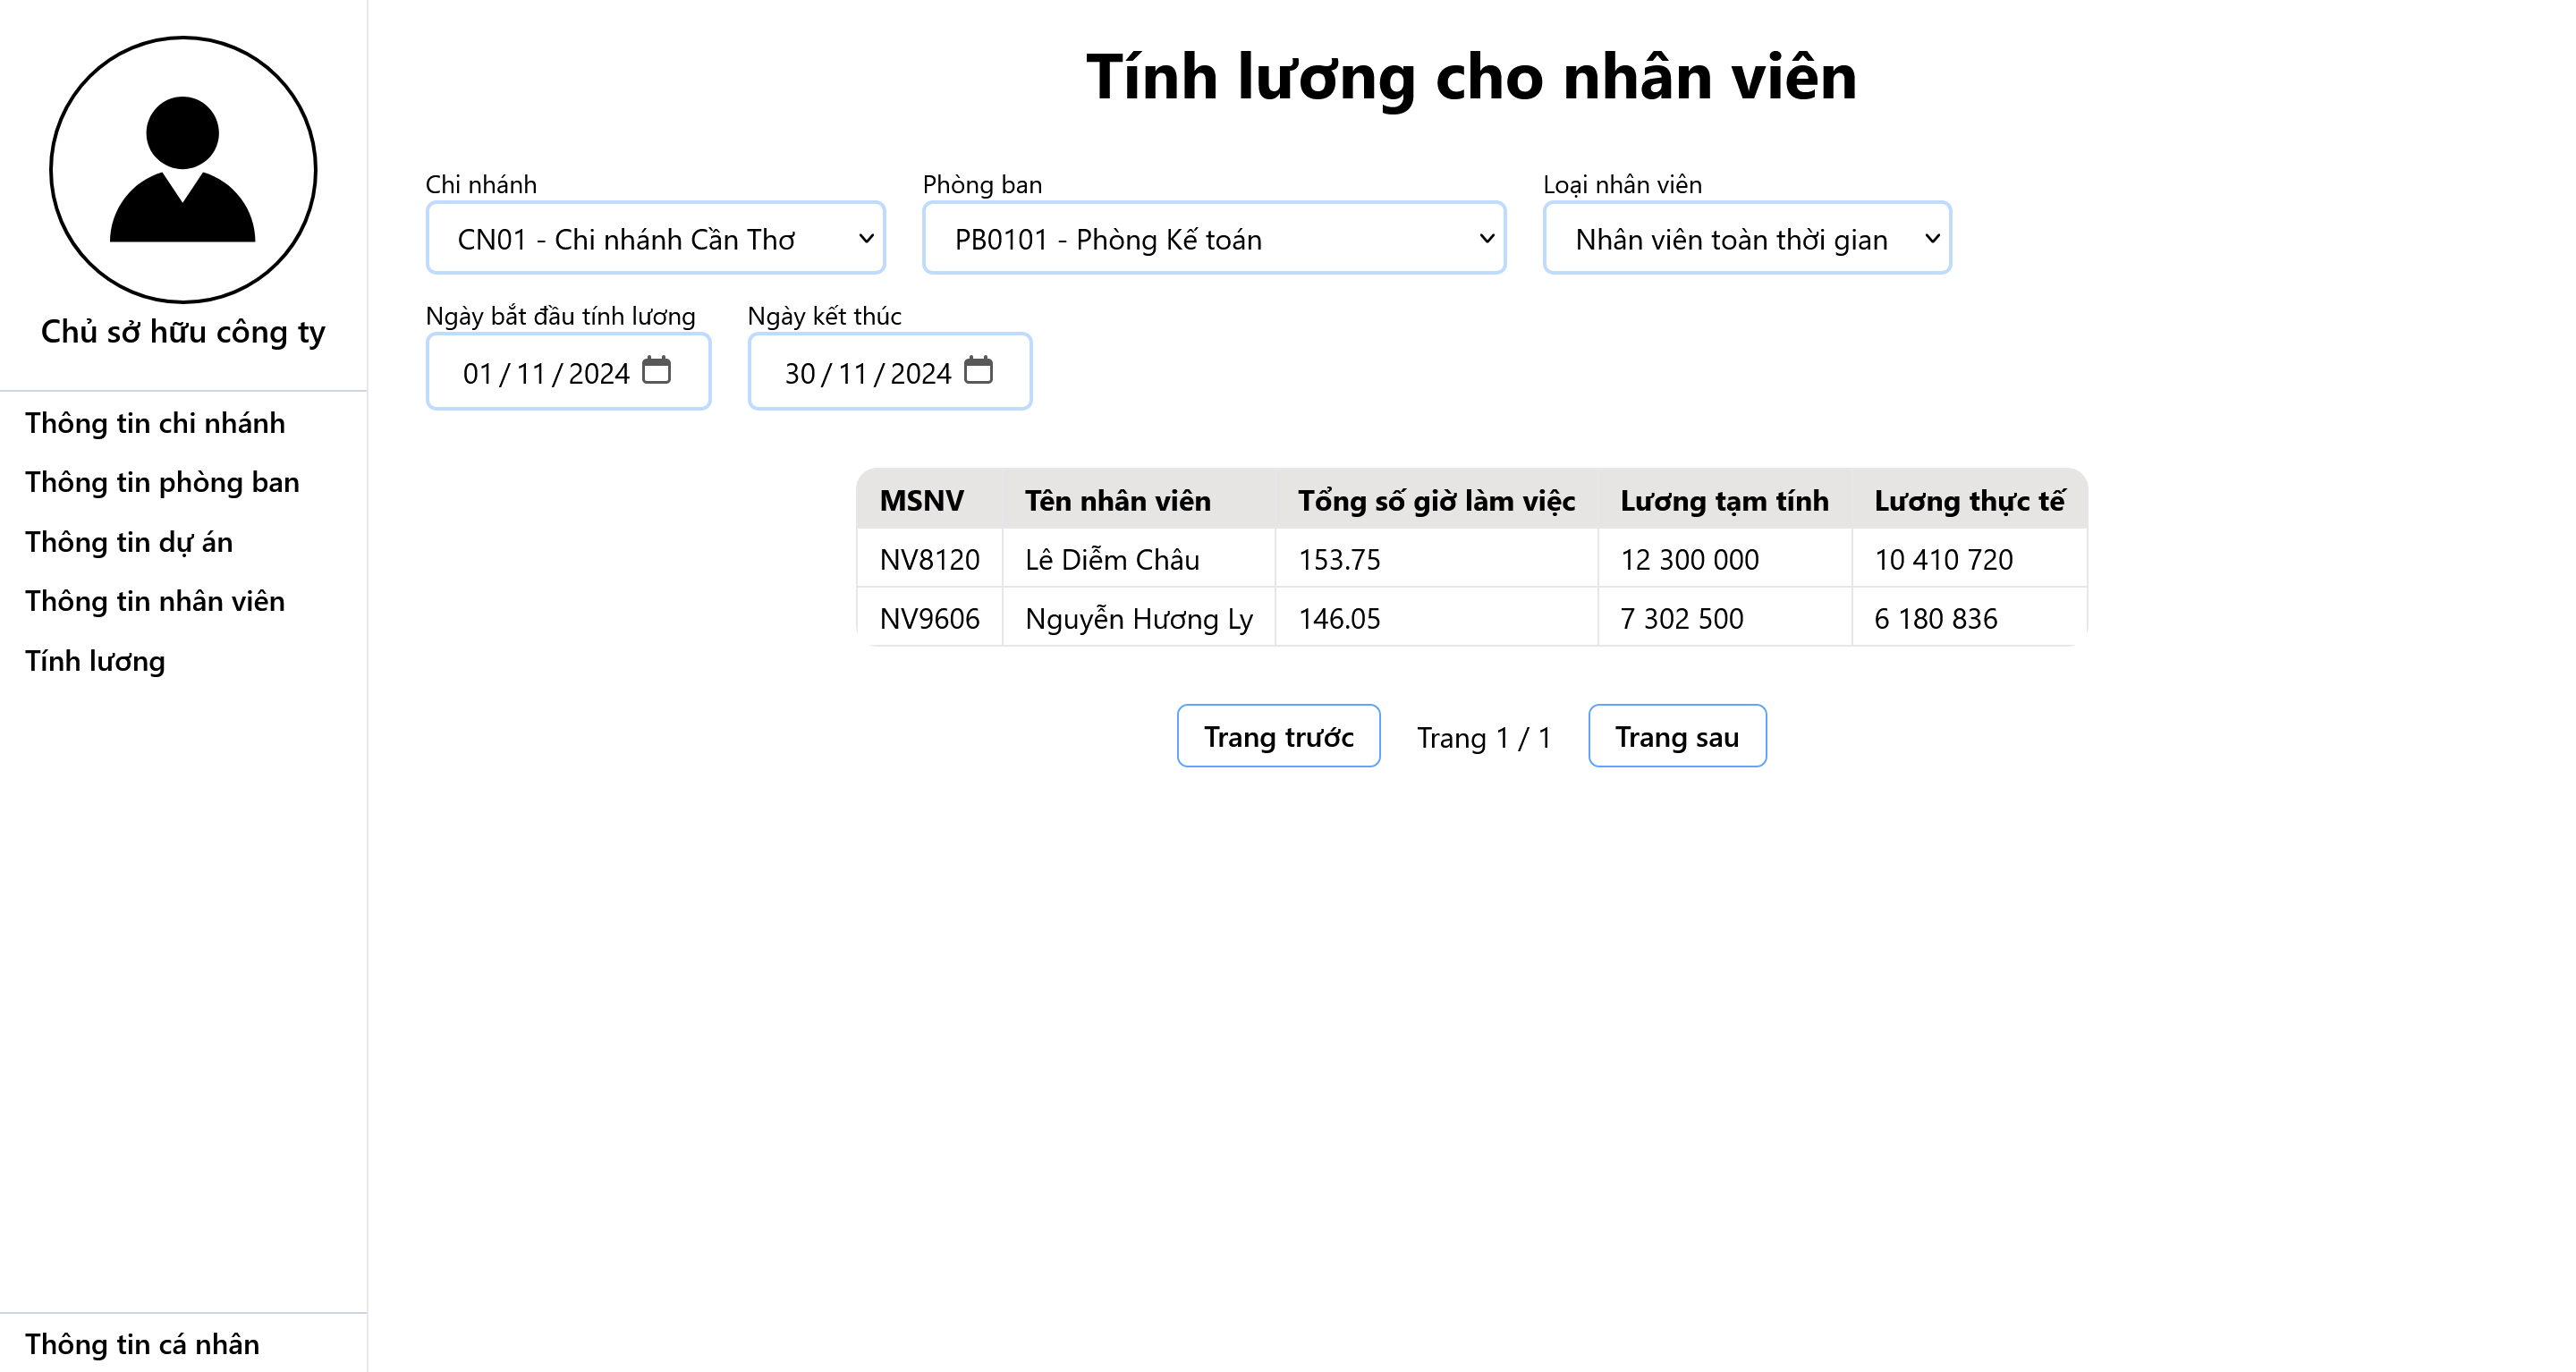
\includegraphics[width=1\linewidth]{content/images/ManHinh_3_d.png}
    \caption{Bảng lương của các nhân viên toàn thời gian thuộc phòng ban '0101'}
    \label{fig:ManHinh_3_d}
\end{figure}

\newpage
Câu lệnh tạo API phục vụ cho màn hình tính lương
\begin{minted}{javascript}
    export const getBangLuong = async (MaPhongBan, EmpType, BeginDate, EndDate) => {
        if ((BeginDate === "") || (EndDate === "")) return [];
        const rows = await ReadFromProcedureQuery(`CALL View_BangLuong('${MaPhongBan}', ${EmpType}, '${BeginDate}', '${EndDate}')`);
        return rows;
    }

    app.get('/api/bang-luong', async (req, res) => {
        let {MaPhongBan, EmpType, BeginDate, EndDate} = req.query;
        if (!MaPhongBan) MaPhongBan = "all";
        try {
            const BangLuong = await getBangLuong(MaPhongBan, EmpType, BeginDate, EndDate);
            // console.log(BangLuong)
            res.status(200).json({
                success: true,
                BangLuong
            })
        } catch (error) {
            console.error(error);
            res.status(500).json({ success: false, message: 'Lỗi server' });
        }
    })
\end{minted}

Component phục vụ việc render dữ liệu:
\begin{minted}{jsx}
    function BangLuong({Data}) {
        const Headers = ["MSNV", "Tên nhân viên", "Tổng số giờ làm việc", "Lương tạm tính", "Lương thực tế"]
        return (
            <Table columnHeaders={Headers} rowsData={Data} />
        )
    }

    export default BangLuong
\end{minted}

Câu lệnh gọi API và render dữ liệu
\begin{minted}{jsx}
    // Khởi tạo các thực thể để lưu giá trị tham số cho câu lệnh gọi API
    const [beginDate, setBeginDate] = useState("")
    const [endDate, setEndDate] = useState("")
    const [maChiNhanh, setMaChiNhanh] = useState("");
\end{minted}
\begin{minted}[firstnumber=5]{jsx}
    const [maPhongBan, setMaPhongBan] = useState("");
    const [empType, setEmpType] = useState(0);
    // Khi người dùng thực hiện việc thay đổi giá trị của các input fields sau, giá trị của các thực thể trên sẽ thay đổi 
    <SelectField label={"Chi nhánh"} placeholder={"Tất cả"} options={chiNhanhOptions} onchangeHandler={handleMaChiNhanh}/>
    <SelectField label={"Phòng ban"} placeholder={"Tất cả"} options={phongBanOptions} onchangeHandler={handleMaPhongBan} />
    <SelectField label={"Loại nhân viên"} placeholder={"Tất cả"} options={["Nhân viên toàn thời gian", "Nhân viên bán thời gian"]} onchangeHandler={handleEmpType}/>
    <InputField label={"Ngày bắt đầu tính lương"} type={'date'} onChangeHandle={handleBeginDate}/>
    <InputField label={"Ngày kết thúc"} type={'date'} onChangeHandle={handleEndDate}/>

    // Khi đã có đầy đủ hai giá trị beginDate và endDate, câu lệnh gọi API sẽ được thực hiện để lấy dữ liệu và lưu vào thực thể bangLuongData
    const [bangLuongData, setBangLuongData] = useState([]);
    const fetchBangLuong = async (maPhongBan, empType, beginDate, endDate) => {
        try {
            const res = await fetch(`api/bang-luong?MaPhongBan=${maPhongBan}&EmpType=${empType}&BeginDate=${beginDate}&EndDate=${endDate}`);
            const data = await res.json();
            console.log(data.BangLuong)
            data.BangLuong.forEach(item => {
                item[3] = numberWithSpaces(item[3])
                item[4] = numberWithSpaces(Math.round(item[4]))
            });
            setBangLuongData(data.BangLuong);
        } catch (error) {
            console.log(error);
        }
    }

    // Dữ liệu đang được lưu ở thực thể bangLuongData sẽ được xử lý để phân trang, các dữ liệu của trang hiện tại sẽ được lưu ở thực thể curData
    const [curData, setCurData] = useState([]);
    useEffect(() => {
        setCurData(bangLuongData.slice(curPage * 10 - 10, curPage * 10));
    }, [bangLuongData, curPage])

    // Cuối cùng, truyền dữ liệu của trang hiện tại xuống component BangLuong để render bảng dữ liệu
    <BangLuong Data={curData}/>
\end{minted}

\newpage